% Options for packages loaded elsewhere
\PassOptionsToPackage{unicode}{hyperref}
\PassOptionsToPackage{hyphens}{url}
%
\documentclass[
]{book}
\title{Mappeeksamen}
\author{Margit Dahl Sørensen}
\date{2021-12-01}

\usepackage{amsmath,amssymb}
\usepackage{lmodern}
\usepackage{iftex}
\ifPDFTeX
  \usepackage[T1]{fontenc}
  \usepackage[utf8]{inputenc}
  \usepackage{textcomp} % provide euro and other symbols
\else % if luatex or xetex
  \usepackage{unicode-math}
  \defaultfontfeatures{Scale=MatchLowercase}
  \defaultfontfeatures[\rmfamily]{Ligatures=TeX,Scale=1}
\fi
% Use upquote if available, for straight quotes in verbatim environments
\IfFileExists{upquote.sty}{\usepackage{upquote}}{}
\IfFileExists{microtype.sty}{% use microtype if available
  \usepackage[]{microtype}
  \UseMicrotypeSet[protrusion]{basicmath} % disable protrusion for tt fonts
}{}
\makeatletter
\@ifundefined{KOMAClassName}{% if non-KOMA class
  \IfFileExists{parskip.sty}{%
    \usepackage{parskip}
  }{% else
    \setlength{\parindent}{0pt}
    \setlength{\parskip}{6pt plus 2pt minus 1pt}}
}{% if KOMA class
  \KOMAoptions{parskip=half}}
\makeatother
\usepackage{xcolor}
\IfFileExists{xurl.sty}{\usepackage{xurl}}{} % add URL line breaks if available
\IfFileExists{bookmark.sty}{\usepackage{bookmark}}{\usepackage{hyperref}}
\hypersetup{
  pdftitle={Mappeeksamen},
  pdfauthor={Margit Dahl Sørensen},
  hidelinks,
  pdfcreator={LaTeX via pandoc}}
\urlstyle{same} % disable monospaced font for URLs
\usepackage{longtable,booktabs,array}
\usepackage{calc} % for calculating minipage widths
% Correct order of tables after \paragraph or \subparagraph
\usepackage{etoolbox}
\makeatletter
\patchcmd\longtable{\par}{\if@noskipsec\mbox{}\fi\par}{}{}
\makeatother
% Allow footnotes in longtable head/foot
\IfFileExists{footnotehyper.sty}{\usepackage{footnotehyper}}{\usepackage{footnote}}
\makesavenoteenv{longtable}
\usepackage{graphicx}
\makeatletter
\def\maxwidth{\ifdim\Gin@nat@width>\linewidth\linewidth\else\Gin@nat@width\fi}
\def\maxheight{\ifdim\Gin@nat@height>\textheight\textheight\else\Gin@nat@height\fi}
\makeatother
% Scale images if necessary, so that they will not overflow the page
% margins by default, and it is still possible to overwrite the defaults
% using explicit options in \includegraphics[width, height, ...]{}
\setkeys{Gin}{width=\maxwidth,height=\maxheight,keepaspectratio}
% Set default figure placement to htbp
\makeatletter
\def\fps@figure{htbp}
\makeatother
\setlength{\emergencystretch}{3em} % prevent overfull lines
\providecommand{\tightlist}{%
  \setlength{\itemsep}{0pt}\setlength{\parskip}{0pt}}
\setcounter{secnumdepth}{5}
\usepackage{booktabs}
\usepackage{booktabs}
\usepackage{longtable}
\usepackage{array}
\usepackage{multirow}
\usepackage{wrapfig}
\usepackage{float}
\usepackage{colortbl}
\usepackage{pdflscape}
\usepackage{tabu}
\usepackage{threeparttable}
\usepackage{threeparttablex}
\usepackage[normalem]{ulem}
\usepackage{makecell}
\usepackage{xcolor}
\usepackage{fontspec}
\usepackage{multicol}
\usepackage{hhline}
\usepackage{hyperref}
\ifLuaTeX
  \usepackage{selnolig}  % disable illegal ligatures
\fi
\usepackage[]{natbib}
\bibliographystyle{plainnat}

\begin{document}
\maketitle

{
\setcounter{tocdepth}{1}
\tableofcontents
}
\hypertarget{rabilitet}{%
\chapter{Rabilitet}\label{rabilitet}}

\hypertarget{introduksjon}{%
\section{Introduksjon}\label{introduksjon}}

Maksimalt oksygenopptak \(\dot VO_{2max}\) ble først beskrevet av
{[}@ \citep{hill1923} , og kan defineres som kroppens evne til å ta opp og
forbruke oksygen per tidsenhet \citep{HillLupton, BassetHowley}. Innen
toppidrett måles ofte det maksimale oksygenopptaket for å måle utøverens
kapasitet opp mot arbeidskravet i den spesifikke idretten, og
\(\dot VO_{2max}\) kan i så måte også sees på som et mål på den aerobe
effekten til utøveren \citep{bassett2000}. I Olympiatoppens testprotokoller
benytter de flere definerte hjelpekriterier for å sikre at man faktisk
har funnet deltakerens maksimale oksygenopptak \citep{tønnessen2017}.
Følgende kriterier er beskrevet; platå i \(\dot VO_{2max}\) er oppnådd,
økning i ventilasjon med utflating av \(\dot VO_{2max}\) verdi, RER over
1.10/1.05, og blodlaktat over 8 \citep{tønnessen2017}

\hypertarget{metode}{%
\section{Metode}\label{metode}}

I forkant av testen målte alle deltakerne kroppsvekten i samme klær som
ble brukt under testen, men ble bedt om å ta av seg skoene. Kroppsvekten
som senere brukt i beregningen av maksimalt oksygenopptak (ml kg\textsuperscript{-1}
min\textsuperscript{-1}) er kroppsvekten målt i forkant av test, etter at 300g har blitt
trukket av for å ta høyde for vekten av klærne. For å sikre intern
validitet ble deltakerne bedt om å avstå fra anstrengende fysisk
aktivitet dagen før test, standardisere måltidet i forkant av test samt
avstå fra inntak av koffein under de siste 12 timene før testen
\citep{halperin2015}. Pre- og post-tester ble gjennomført på samme tid på
døgnet under standardiserte forhold.. Post-test ble gjennomført 6 dager
etter gjennomført
pretest.
Det ble ikke kontrollert for fysisk aktivitet mellom testdagene.

Alle deltakerne gjennomførte en 10 minutter lang oppvarmingsprotokoll på
tredemøllen (Woodway, 4 front , Wisconsin), beskrevet for deltakerne i
forkant av testen. Denne oppvarmingsprotokollen bestod av fem minutter
på 11-13 i Borg 6-20 RPE skala (Borg,1982),
etterfulgt av 2x1min på starthastighet og stigning med 30 sekund
mellom.
Siste tre min var også 11-13 i
borg. Etter oppvarming
var det to min pause før testen begynte. Starthastighet for begge
kjønn var satt til
8km/t, med stigning på 10.5\% og 5.5\% for henholdsvis menn og kvinner.

̇VO2max ble målt ved hjelp av en metabolsk analysator med
Vyntus CPX miksekammer (Vyntus CPX, Jaeger-CareFusion, UK). Forut for
alle tester ble analysatoren gass og volumkalibrert med en feillmargin
på henholdsvis 2\% og 0.2\%. Analysatoren ble
stilt inn til å gjøre målinger hvert 30sek, og V̇O\textsubscript{2max} ble kalkulert
gjennom å bruke snittet av de to høyeste påfølgende målingene av V̇O\textsubscript{2}.
Underveis i testen mottok alle deltakerne en høylytt verbal oppmuntring
fra testleder. Alle deltakerne
gjennomførte også begge testene med samme testleder og med samme
personer til stede i rommet for å redusere konfundering \citep{halperin}.

For hvert medgåtte minutt av testen ble hastigheten på møllen økt med
1km/t, helt til utmattelse, hvor testen ble avsluttet. Deltakernes
hjertefrekvens (GARMIN/POLAR) ble også registrert under hele testen. Når
testen ble avsluttet ble deltakerne bedt om å rapportere opplevd
anstrengelse ved hjelp av Borg-skala \citep{borg1982}. Maksimal
hjertefrekvens under testen ble også registrert. Ett minutt etter
avsluttet test ble hjertefrekvens registrert, og det ble målt og
analysert blodlaktat(BIOSEN).

\hypertarget{resultater}{%
\section{Resultater}\label{resultater}}

\providecommand{\docline}[3]{\noalign{\global\setlength{\arrayrulewidth}{#1}}\arrayrulecolor[HTML]{#2}\cline{#3}}

\setlength{\tabcolsep}{2pt}

\renewcommand*{\arraystretch}{1.5}

\begin{longtable}[c]{|p{1.08in}|p{1.02in}|p{1.02in}}



\hhline{>{\arrayrulecolor[HTML]{666666}\global\arrayrulewidth=2pt}->{\arrayrulecolor[HTML]{666666}\global\arrayrulewidth=2pt}->{\arrayrulecolor[HTML]{666666}\global\arrayrulewidth=2pt}-}

\multicolumn{1}{!{\color[HTML]{000000}\vrule width 0pt}>{\raggedright}p{\dimexpr 1.08in+0\tabcolsep+0\arrayrulewidth}}{\fontsize{11}{11}\selectfont{\textcolor[HTML]{000000}{\global\setmainfont{Helvetica}{}}}} & \multicolumn{1}{!{\color[HTML]{000000}\vrule width 0pt}>{\raggedright}p{\dimexpr 1.02in+0\tabcolsep+0\arrayrulewidth}}{\fontsize{11}{11}\selectfont{\textcolor[HTML]{000000}{\global\setmainfont{Helvetica}{Kvinner}}}} & \multicolumn{1}{!{\color[HTML]{000000}\vrule width 0pt}>{\raggedright}p{\dimexpr 1.02in+0\tabcolsep+0\arrayrulewidth}!{\color[HTML]{000000}\vrule width 0pt}}{\fontsize{11}{11}\selectfont{\textcolor[HTML]{000000}{\global\setmainfont{Helvetica}{Menn}}}} \\

\noalign{\global\setlength{\arrayrulewidth}{2pt}}\arrayrulecolor[HTML]{666666}\cline{1-3}

\endfirsthead

\hhline{>{\arrayrulecolor[HTML]{666666}\global\arrayrulewidth=2pt}->{\arrayrulecolor[HTML]{666666}\global\arrayrulewidth=2pt}->{\arrayrulecolor[HTML]{666666}\global\arrayrulewidth=2pt}-}

\multicolumn{1}{!{\color[HTML]{000000}\vrule width 0pt}>{\raggedright}p{\dimexpr 1.08in+0\tabcolsep+0\arrayrulewidth}}{\fontsize{11}{11}\selectfont{\textcolor[HTML]{000000}{\global\setmainfont{Helvetica}{}}}} & \multicolumn{1}{!{\color[HTML]{000000}\vrule width 0pt}>{\raggedright}p{\dimexpr 1.02in+0\tabcolsep+0\arrayrulewidth}}{\fontsize{11}{11}\selectfont{\textcolor[HTML]{000000}{\global\setmainfont{Helvetica}{Kvinner}}}} & \multicolumn{1}{!{\color[HTML]{000000}\vrule width 0pt}>{\raggedright}p{\dimexpr 1.02in+0\tabcolsep+0\arrayrulewidth}!{\color[HTML]{000000}\vrule width 0pt}}{\fontsize{11}{11}\selectfont{\textcolor[HTML]{000000}{\global\setmainfont{Helvetica}{Menn}}}} \\

\noalign{\global\setlength{\arrayrulewidth}{2pt}}\arrayrulecolor[HTML]{666666}\cline{1-3}\endhead



\multicolumn{3}{!{\color[HTML]{FFFFFF}\vrule width 0pt}>{\raggedright}p{\dimexpr 3.13in+4\tabcolsep+2\arrayrulewidth}!{\color[HTML]{FFFFFF}\vrule width 0pt}}{\fontsize{11}{11}\selectfont{\textcolor[HTML]{000000}{\global\setmainfont{Helvetica}{Verdier\ er\ gitt\ som\ gjennomsnitt\ og\ (Standardavvik)}}}} \\

\endfoot



\multicolumn{1}{!{\color[HTML]{000000}\vrule width 0pt}>{\raggedright}p{\dimexpr 1.08in+0\tabcolsep+0\arrayrulewidth}}{\fontsize{11}{11}\selectfont{\textcolor[HTML]{000000}{\global\setmainfont{Helvetica}{N}}}} & \multicolumn{1}{!{\color[HTML]{000000}\vrule width 0pt}>{\raggedright}p{\dimexpr 1.02in+0\tabcolsep+0\arrayrulewidth}}{\fontsize{11}{11}\selectfont{\textcolor[HTML]{000000}{\global\setmainfont{Helvetica}{4}}}} & \multicolumn{1}{!{\color[HTML]{000000}\vrule width 0pt}>{\raggedright}p{\dimexpr 1.02in+0\tabcolsep+0\arrayrulewidth}!{\color[HTML]{000000}\vrule width 0pt}}{\fontsize{11}{11}\selectfont{\textcolor[HTML]{000000}{\global\setmainfont{Helvetica}{7}}}} \\





\multicolumn{1}{!{\color[HTML]{000000}\vrule width 0pt}>{\raggedright}p{\dimexpr 1.08in+0\tabcolsep+0\arrayrulewidth}}{\fontsize{11}{11}\selectfont{\textcolor[HTML]{000000}{\global\setmainfont{Helvetica}{Alder\ (år)}}}} & \multicolumn{1}{!{\color[HTML]{000000}\vrule width 0pt}>{\raggedright}p{\dimexpr 1.02in+0\tabcolsep+0\arrayrulewidth}}{\fontsize{11}{11}\selectfont{\textcolor[HTML]{000000}{\global\setmainfont{Helvetica}{24.5\ (1.29)}}}} & \multicolumn{1}{!{\color[HTML]{000000}\vrule width 0pt}>{\raggedright}p{\dimexpr 1.02in+0\tabcolsep+0\arrayrulewidth}!{\color[HTML]{000000}\vrule width 0pt}}{\fontsize{11}{11}\selectfont{\textcolor[HTML]{000000}{\global\setmainfont{Helvetica}{23.9\ (1.77)}}}} \\





\multicolumn{1}{!{\color[HTML]{000000}\vrule width 0pt}>{\raggedright}p{\dimexpr 1.08in+0\tabcolsep+0\arrayrulewidth}}{\fontsize{11}{11}\selectfont{\textcolor[HTML]{000000}{\global\setmainfont{Helvetica}{Vekt\ (kg)}}}} & \multicolumn{1}{!{\color[HTML]{000000}\vrule width 0pt}>{\raggedright}p{\dimexpr 1.02in+0\tabcolsep+0\arrayrulewidth}}{\fontsize{11}{11}\selectfont{\textcolor[HTML]{000000}{\global\setmainfont{Helvetica}{58.9\ (6.28)}}}} & \multicolumn{1}{!{\color[HTML]{000000}\vrule width 0pt}>{\raggedright}p{\dimexpr 1.02in+0\tabcolsep+0\arrayrulewidth}!{\color[HTML]{000000}\vrule width 0pt}}{\fontsize{11}{11}\selectfont{\textcolor[HTML]{000000}{\global\setmainfont{Helvetica}{74.8\ (5.55)}}}} \\





\multicolumn{1}{!{\color[HTML]{000000}\vrule width 0pt}>{\raggedright}p{\dimexpr 1.08in+0\tabcolsep+0\arrayrulewidth}}{\fontsize{11}{11}\selectfont{\textcolor[HTML]{000000}{\global\setmainfont{Helvetica}{Høyde\ (cm)}}}} & \multicolumn{1}{!{\color[HTML]{000000}\vrule width 0pt}>{\raggedright}p{\dimexpr 1.02in+0\tabcolsep+0\arrayrulewidth}}{\fontsize{11}{11}\selectfont{\textcolor[HTML]{000000}{\global\setmainfont{Helvetica}{166\ (2.99)}}}} & \multicolumn{1}{!{\color[HTML]{000000}\vrule width 0pt}>{\raggedright}p{\dimexpr 1.02in+0\tabcolsep+0\arrayrulewidth}!{\color[HTML]{000000}\vrule width 0pt}}{\fontsize{11}{11}\selectfont{\textcolor[HTML]{000000}{\global\setmainfont{Helvetica}{180\ (3.1)}}}} \\

\noalign{\global\setlength{\arrayrulewidth}{2pt}}\arrayrulecolor[HTML]{666666}\cline{1-3}



\end{longtable}

Det var 11 deltakere i studien, samtlige deltakere er studenter ved
Høgskolen i Innlandet. Deskriptive data for disse deltakerne er vist i
Tabell 1, i Figur 1 kan man se utviklingen fra pre-test til post-test
fordelt på kjønn. Det typiske målefeilet (typical error, \citep{hopkins}) fra
pre til post-test er utregnet til å være 4.04\%.

\begin{figure}
\centering
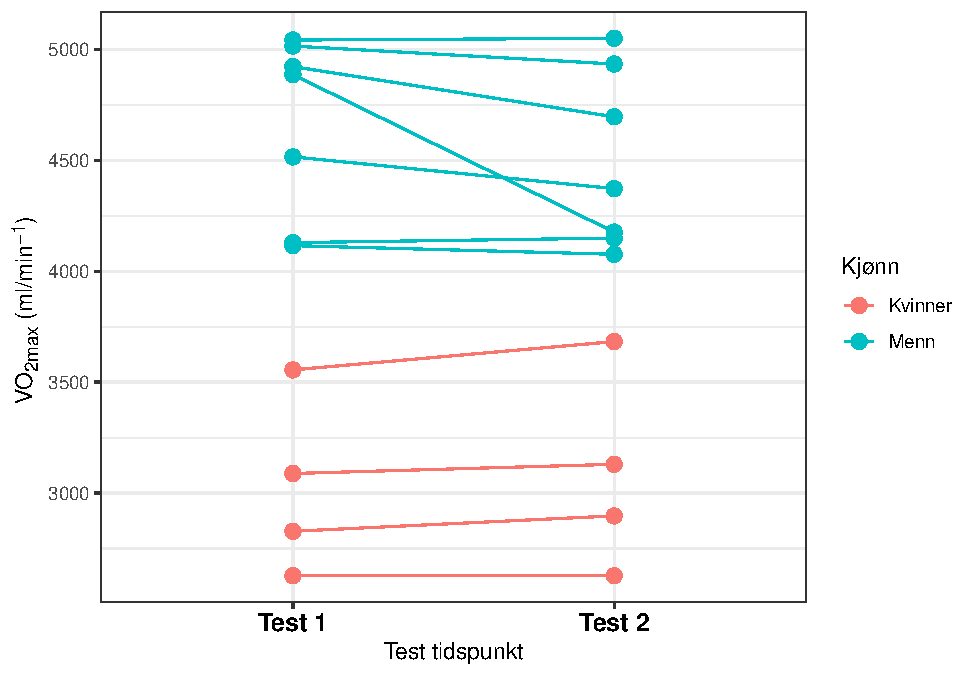
\includegraphics{_main_files/figure-latex/unnamed-chunk-3-1.pdf}
\caption{\label{fig:unnamed-chunk-3}Figurtekst legg til\ldots{}}
\end{figure}

\hypertarget{diskusjon}{%
\section{Diskusjon}\label{diskusjon}}

Ettersom testing av maksimalt oksygenopptak er en test som gjennomføres
til utmattelse, vil man kunne forvente en viss variasjon i
testresultatene ettersom opplevd anstrengelse kan påvirkes av flere
ulike variabler \citep{halperin2015}. For å redusere
konfundering
vil flere faktorer være nyttig å ta hensyn til under slik testing. Som
nevnt i metoden vil standardisering av matinntak, koffeininntak, utstyr
og tidspunkt for gjennomføring av test være med på å kunne sikre intern
validitet i resultatene. Eksempler er deltakernes kjennskap til testen,
verbal oppmuntring og personer tilstede under testen er andre faktorer
som potensielt kan bidra til konfundering. Felles for alle faktorer er
at graden av påvirkning på resultatene muligens reduseres ved hjelp av
en standardisert testprotokoll. Deltakerne - og testlederne, sin
kjennskap til testen er en annen faktor som trolig påvirker resultatene
i vårt prosjekt. I dette tilfellet fantes det enkelte deltakere som
hadde gjennomført en liknende test flere ganger, og en kan da forvente
en mindre grad av variasjon mellom resultatene på pre og post test,
sammenlignet med de deltakerne som gjennomførte testen for første gang
på pretest. Dette fordi kjennskapen og kunnskapen de tilegnet seg på
pre-test, trolig spiller inn på testresultatene.
Standardfeilen
på 4.04\% kan også tyde på at enkelte av disse resultatene kan være
utsatt for konfundering av ulik sort \citep{hopkins2000}.

Grunnen til at vi snakker om standardfeil er at når vi ønsker å måle
påvirkningen av trening på en gruppe individer er det viktig å kunne si
noe om hva som er endring og hva som er støy (målefeil). Desto mindre
støy en test innebærer jo bedre er målingen. Målet som brukes er
standardfeil. Hva som danner denne variasjonen som representeres ved
typical error er multifaktorelt, men hoveddelen er som oftest biologisk
\citep{hopkins2000}.

For å måle standardfeil har vi brukt within subject deviation metoden.
Denne metoden påvirkes ikke av at gjennomsnittet endrer seg fra test til
test \citep{hopkins2000} . Data for målinger i VO2max fra fem sertifiserte
Australske laboratorier fastslo ett gjennomsnitt på 2.2\% for
standardfeil \citep{halperin2015}. Data fra det Australske institutt for
sport har også fastslått at en standardfeil på omtrent 2\% er riktig for
både maksimal og submaksimal VO2 \citep{clark2007, robertson2010, saunders2009}. Dette indikerer at med godt kalibrert utstyr og med
utøvere som er godt vant med testingen vil en standardfeil på 2\% for det
biologiske, og analytiske være riktig \citep{halperin2015}. Vår standardfeil
på 4.04\% kan derfor tenkes å være et bilde hvordan det kan se ut med få
deltakere, med ulikt utgangspunkt, men også uten skikkelig
standardisering av treningshverdagen i forkant av testene. Det kan også
tenkes at med et varierende nivå hos deltagerne kan enkelte oppleve en
treningseffekt av test 1. Samtidig som andre kanskje ble slitne av å få
en test inn i treningshverdagen.

\hypertarget{referanser}{%
\section{Referanser}\label{referanser}}

\hypertarget{labrapport}{%
\chapter{Labrapport}\label{labrapport}}

\hypertarget{formuxe5l}{%
\section{Formål}\label{formuxe5l}}

\hypertarget{arbeidskrav-i-vitenskapsteori}{%
\chapter{Arbeidskrav i vitenskapsteori}\label{arbeidskrav-i-vitenskapsteori}}

\hypertarget{oppgave-1}{%
\section{Oppgave 1}\label{oppgave-1}}

Falsifikasjonisme Karl Popper var en analytisk filosof, som utarbeidet et falsifiserbarhetskriterium. Popper ble inspirert til denne tankegangen gjennom tre ulike kilder, demarkasjonsproblemet, induksjonsproblemet og risikable forutsigelser. Demarkasjonsproblemet danner grunnlaget for utfordringen med å skille vitenskap og pseudovitenskap fra hverandre. Induksjonsproblemet stiller et spørsmål om hvordan man kan vite at en vitenskapelig teori er sann. Dette så ikke Popper på som et problem da han mente at vitenskapelige teorier ikke kan bekreftes. Det siste som inspirerte popper er risikable forutsigelser som er vanskelig eller umulige å falsifisere \citep{alnes2018}.

Poppers demarkasjonskriterium kommer fra ønsket å skille vitenskapelig teori fra ikke-vitenskapelig teori også kalt pseudovitenskap \citep{dellsén2021}. Løsningen på dette mente han ikke kunne komme fra å verifisere teorier, da dette kan være vanskelig eller umulig. Løsningen på dette problemet blir da å falsifisere teorier, ergo å bekrefte at de er usanne, eller feil. Et eksempel på dette er en teori om at alle hunder er hvite. Det er umulig å bekrefte at det aldri har vært hunder som har en annen farge, eller at det noen gang kommer til å være hunder som har en annen farge. Dette er årsaken til at Popper mener det er umulig å bekrefte en teori, da man aldri kan vite hva som har vært eller hva som kommer. Ved å bruke samme eksempel kan man falsifisere teorien når man oppdager en hund som ikke er hvit. Falsifikasjon er da kriteriet som kan skille vitenskap fra pseudovitenskap, i følge Popper \citep{okasha2016}.

Popper ytret at vitenskapelige teorier som ikke er mulig å falsifisere, hvor man uansett kan få de empiriske bevisene til å passe inn i teorien, skaper lite troverdighet og at disse ikke skulle godtas som vitenskapelig teori \citep{okasha2016}. Popper \citep{popper1969} forklarer dette med teorier fra Marx, Freud og Adler, som han syns var utfordrende at skulle aksepteres som vitenskapelige teorier. Teorier som er mulig å falsifisere (dette betyr ikke at de trenger å være usanne) er mer troverdig, og viktige teorier når de blir testet.

Samir Okasha \citep{okasha2016} beskriver flere utfordringer ved Poppers falsifiserbarhetskriterium. En av utfordringene Okasha beskriver er hvordan dette kriteriet kan påvirke hvordan verden blir oppfattet hvis man hele tiden skal avkrefte teorier. Med dette mener han at vitenskapelige teorier som ikke kan falsifiseres likevel kan ha eller hatt stor påvirkning på hvordan den vitenskapelige teoriene kan utvikle seg. Disse teoriene kan og bidra til nye viktige oppdagelser innenfor tematikken. Videre beskriver Okasha problematikken med å skulle definere hvile teorier som kan kalles vitenskap og ikke-vitenskap, og hvorfor dette ikke er nødvendig. Et av eksemplene han trekker frem er hvordan det nesten er umulig at alle observasjoner stemmer med en vitenskapelig teori. Videre beskriver han hvor vid og bred vitenskapen er, og hvor ulik alle teoriene er. Han beskriver vitenskap som ulike teorier som har mange fellestrekk, og at selv uten alle fellestrekkene vil dette være vitenskapelige teorier med bekreftende observasjoner \citep{okasha2016}. Jeg mener Okasha har et godt poeng i at det ikke er så viktig å skille mellom vitenskap og psudovitenskap som Popper ønsket. Som Okasha påpeker har det blitt gjort viktig oppdagelser i lyset av en teori som viste seg å ikke stemme, og det er derfor ikke like viktig med det markante skillet, men at begrepet er litt flytende.

\hypertarget{oppgave-2}{%
\section{Oppgave 2}\label{oppgave-2}}

HD-metoden og abduksjon/Bayesisme Hypotetisk deduktiv metode kan deles i to ulike kontekster for ulike faser av utvikling av teorien, oppdagelseskonteksten og begrunnelseskonteksten. Oppdagelseskonteksten er miljøet der teorien eller hypotesen blir oppdaget. I følge Hempel finnes det ingen bestemt metode å finne opp nye ideer, men de kan for eksempel oppstå fra fantasier eller ulike observasjoner man gjør \citep{dellsén2021}. Dette kan forekommer tilfeldig, eller hvis man prøver å finne en forklaring eller årsak på et bestemt problem. Dette er begrunnelseskonteksten. Hempel \citep{hempel1966} beskriver at det ikke er noen fasit på hvordan nye teorier blir oppdaget, men at det skje på mange ulike måter.

Den logiske strukturen i hypotetisk deduktiv metode er å bekrefte om en idé stemmer ved å teste den, gjennom å observere konsekvensene. Metoden er delt inn i fire ulike faser for bekreftelse av en ny teori \citep{dellsén2021}. Fase en er å oppdage en ny teori eller lete etter en hypotese på et problem. Andre fase er å dedusere de empiriske konsekvensene fra teorien. Dette vil si at hypotesen kan være «det finnes liv på Jupiter». Dette vil si at de empiriske konsekvensene av dette vil være at det er oksygen på Jupiter, det er vann på Jupiter osv. Ved fase 3 undersøker man, og samler inn data for å se om hypotesen stemmer, og om innsamlede data stemmer med de empiriske konsekvensene. For eksempelet beskrevet over vil dette bety at man må teste om det er oksygen, vann osv på Jupiter. Hvis de ikke stemmer forkaster man, eller endre hypotesen for å komme nærmere en ny idé eller hypotese som forklarer problemstillingen. Når man eventuelt har innsamlede data som stemmer med de empiriske konsekvensene kan man konkludere. Da har man til en viss grad fått en induktiv bekreftelse av hypotesen. Dette fordi det kan være andre årsaker som fører til endringen eller årsakssammenheng som hypotesen ikke tar for seg. Dette vil ikke bety at den hypotesen som man først har kommet frem til ikke stemmer, men at det er andre årsaksforhold som og kan påvirke \citep{hempel1966}.

Abduksjon er en vitenskapelig metode man bruker for å bekrefte teorier. Denne metoden handler om å dra slutninger til den beste forklaringen til et nytt fenomen eller ny data. For å finne dette trenger man flere ulike teorier som har forskjellige årsaksforklaringer på dataen. Det er flere elementer som kan bidra til at en forklaring er bedre. Hvis teorien har forklaringskraft, forklarer flere forskjellige data, vil dette styrke teorien. Det samme gjelder hvis teorien har en enklere årsaksforklaring, forklarer dataen ut fra færre ting \citep{dellsén2021}. Dette vil si at i abduksjon må man sammenligne flere ulike forklaringer til samme fenomen, og finne den som best forklarer dataen.

For å sammenligne med hypotetisk deduksjon som oppgir en hypotese med ulike empiriske konsekvenser tilbyr abduksjon flere hypoteser eller forklaringer. Noe som kan være en svakhet med HD metoden er at det kan være flere konsekvenser og årsaker som kan underligge ved en «korrekt» hypotese enn det man ser. En annen svakhet med HD metoden er at svarene man får fra dataen kan være en tilfeldighet, som gjør at det virker som man bekrefter hypotesen, men det er egentlig andre bedre forklaringer på problemet. Dette er et av problemene som gjorde at abduksjon ble skapt. Ved abduksjon ønsker man å se på ulike forklaringer og finne den metoden som gir den beste forklaringen til problemet. Dette betyr at det abduksjon ønsker å se flere forklaringene til det samme problemet for å finne den beste forklaringen \citep{dellsén2021}.

\hypertarget{oppgave-3}{%
\section{Oppgave 3}\label{oppgave-3}}

Bird beskriver replikasjonskrisen som foregår innenfor forskningsfeltet, som et stort problem som kan ha flere negative konsekvenser for vitenskapelig allmenhet, som at troverdigheten er synkende. Bird bruker tre ulike konsept for å forklare replikasjonskrisen. Disse er type-I feil, type-II feil og basefrekvensfeilen. Type-I feil, er å akseptere en hypotese eller teori som ikke stemmer \citep{bird2020}. Et eksempel på dette kan være en promilletest som viser at en sjåfør kjører med promille, selv om sjåføren ikke har drukket alkohol. Type-II feil er å forkaste en hypotese eller en teori som faktisk stemmer. Dette kan være at en promille test viser at en påvirket sjåfør ikke har promille. Basefrekvensfeilen er en feil som forekommer når man fokuserer på at en viss sannsynlighet forekommer ved en test, som å se på hvor mange sjåfører som kjører ruspåvirket. Hvis 50 av 1000 mennesker som blir testet for rus, tester positivt, men bare 10 faktisk kjørte ruspåvirket, vil det si at det var 40 falsk-positive tester. Fenomenet påpeker da at når man konkluderer med hvor mange tester som slo ut for rus, og ikke tar hensyn for hvor mange falsk-positive tester det var forekommer basefrekvensfeilen. Det er færre folk som ikke kjører påvirket, så da er sannsynligheten for at de daller i den 5\% feilen større enn at de faktisk kjører ruspåvirket. I dette eksempelet vil basefrekvensfeilen oppstå fordi frekvensen av ruspåvirket sjåfører mot ikke-ruspåvirket sjåfører i befolkningen generelt er lav. Bird påpeker hvordan dette slår ut i forskning ved å bruke dette fenomenet. Satt i sammenheng med forskning viser Bird til hvordan dette vil slå ut på hypotesetesting, og hvordan falsk-positive, og falsk-negative forkastninger vil forekomme. Dette fordi man ikke tar høyde for den generelle forekomsten i befolkningen når man tester på for små grupper \citep{bird2020}.

En annen forklaringer som blir nevnt ved replikasjonskrisen er publikasjons bias. Publikasjons bias forekommer når resultater blir skjevt fremstilt for å avgjøre om en studie skal publiseres eller ikke. Dette forekommer først og fremst ved å oftere publisere studier med statistisk signifikante resultater. Dette vil da bety at studier som er gjennomført hvor resultatene ikke er statistisk signifikante, resultatene ikke stemmer med hypotesen ikke vil bli publisert \citep{bird2020}.

Andre forklaringer til replikasjonskrisen er at flere studier ikke blir gjennomført på tilstrekkelig måte for å kunne repetere forsøket, eller at studiet mangler validitet, ergo at studiet ikke gjennomføres på den måten det var planlagt at det skulle gjøres, eller gjennomført slik det er beskrevet at det er gjort. En annen forklaring som blir nevnt er hacking av resultater for å få en studie til å se bedre ut enn det er \citep{bird2020}.

Bird presenterer en mer akademisk forklaring enn de andre årsakene som blir nevnt. Om forskere driver med svindel eller praktiserer dårlig gjennomføring i studiene blir vanskelig å kunne konkludere med. Bird kommer med en forklaring som viser hvordan hypotesetesting kan tolkes feil, eller aksepteres med stor mulighet for type-I eller type-II feil. Forklaringene som har blitt nevnt er alle aksepterbare, og mulige, og det blir vanskelig å konkludere at den ene er bedre enn den andre, men Bird presenterer en mer troverdig forklaring.

\hypertarget{referanser-1}{%
\section{Referanser}\label{referanser-1}}

\hypertarget{styrke-og-utholdenhetstrening-for-godt-trente-syklister}{%
\chapter{Styrke og utholdenhetstrening for godt trente syklister}\label{styrke-og-utholdenhetstrening-for-godt-trente-syklister}}

Styrketrening og utholdenhetstrening for godt trente syklister Introduksjon I denne oppgaven skal jeg se på fem ulike forskningsartikler som undersøke hvilken effekt styrketrening, i tillegg til utholdenhetstrening, har på godt trente syklister. Disse fem artiklene har jeg valgt på bakgrunn av at alle ser på hvilken effekt styrketrening har på prestasjon i sykkel, og hvordan de har brukt ulike metoder og tester for å vise resultatet.

\hypertarget{metode-1}{%
\section{Metode}\label{metode-1}}

\underline{\textbf{Hypotese}} Litteraturen som er valgt til denne oppgaven har alle som hovedmål å undersøke hvordan tung styrketrening i tillegg til vanlig utholdenhetstrening vil påvirke ulike prestasjonsfaktorer innenfor sykling. Hvilke prestasjonsfaktorer som blir vektlagt varierer mellom de ulike forskningsartiklene. Rønnestad \citep{rønnestad2010b} presenterer sin hypotese at styrketreningen vil påvirke muskeltverrsnitt i lårmuskulaturen, power output, windgate test, og 40 min all-out test. Vikmoen et al \citep{vikmoen2016} presenterer samme hypotese, men studien gjennomføres kun på kvinnelige elitesyklister. I artikkelen fra \citep{rønnestad2010a} har Rønnestad et al en hypotese om at vedlikehold av tung styrketrening gjennom starten av treningssesongen vil positivt påvirke utholdenheten over lengre konkurranser i slutten av en 13 ukers periode. Dette minne om hypotesen Aagaard 2011 legger frem, men intervensjonen og resultater blir gjennomført i forberedelses sesong, og ikke i konkurransesesong. Siste artikkel har en hypotese som sier at 10 uker med tung styrketrening sammen med utholdenhetstrening, og 15 uker med vedlikehold av styrketreningen vil gi økt styrke i pedaltråkk og øke styrken i benmuskulaturen \citep{rønnestad2015}.

\underline{\textbf{Studie design}}

Forskningsartiklene som er brukt i denne oppgaven har som hovedmål å finne ut hvordan styrketrening, sammen med utholdenhetstrening, påvirker profesjonelle eller godt trente syklisters prestasjon. Felles for alle studiene er at de gjennomføre en styrkeintervensjon fra 11 til 25 uker på intervensjonsgruppene, og sammenligner forskjellene i ulike styrke- og utholdenhetstester med en kontrollgruppe. De sammenligner Dette vil si at alle studiene bruker randomisert kontrollert studie \citep[RCT{]} som studiedesign. I et RCT blir deltakerne tilfeldig valgt hvilken gruppe de tilhører, kontrollgruppe eller intervensjonsgruppe. Ved å tilfeldig fordele de ulike deltakerne i kontrollgruppe, og intervensjonsgruppe vil man minske sannsynligheten for at det er store forskjeller mellom gruppene \[@hulley2013; @Parab2010\]. Det er med fordel at alle studiene i denne oppgaven bruker dette studie designet for å kunne se effekten for intervensjonsgruppen, mot kontrollgruppen. Dette vil si at resultatene vil vise hvilken effekt intervensjonen har eller ikke har, og ikke være påvirket av store gruppeforskjeller \[@helsebiblioteketuå\] . Utvalg: I de ulike studiene skilte deltaker gruppene seg fra 12 til 23 deltakere. Alle deltakerne var godt trente syklister. I noen av prosjektene var deltakerne syklister på høyt nasjonalt eller internasjonalt nivå {[}][]{rønnestad2010a, rønnestad2010b, rønnestad2015, aagaard2011}. Ingen av forfatterne beskrev rekrutteringsprosessen eller at det ble gjennomført en styrkeberegning (antall beregning) for å argumentere for antall deltakere i studiene.

\underline{\textbf{Tester}}

Alle forskningsprosjektene gjennomført av Rønnestad \citep{rønnestad2010a, rønnestad2010b, rønnestad2015} gjennomfører de samme fysiske testene for å teste intervensjonsgruppen mot kontrollgruppen. Disse testene er beskrevet i tabell 1. Vo2 maks test, windgate og 40 min all-out test ble brukt i prosjektet gjennomført av Vikmoen \citep{vikmoen2016}. I det siste prosjektet ble det gjennomført en 5 min prestasjonstest for å se på effekten av intervensjonen ved kort utholdenhetsprestasjon \citep{aagaard2011}. Det ble og gjennomført en 45 min utholdenhetstest. Felles for alle forskningsprosjektene er at testene var standardisert, for å øke validiteten. Deltakerne måtte følge visse regler under testdagene slik at de eksterne faktorene skulle være så like som mulige. Dette innebar regulasjoner på inntak av mat og drikke, og trening under testdagene. Testtidspunkt var standardisert til den enkelte deltaker, slik at testene ble gjennomført likt på dagen, og temperaturen i testrommet var standardisert på alle utøverne.

De ulike artiklene har brukt forskjellige statistiske tester, for å regne ut forskjellen mellom gruppene. For å regne ut forskjellen mellom gruppene ved pre-test har fire av prosjektene brukt uparret t-test \citetext{\citealp{rønnestad2010a}; \citealp{rønnestad2010b}; \citealp{rønnestad2015}; \citealp[. En t-test blir brukt for å regne ut om det er signifikant forskjell mellom gjennomsnittet til to grupper. I disse studiene er t-testen brukt på to uavhengige grupper, som gjør at man må bruke en uparet t-test \citet{kim2015} . I motsetning til de andre har Aagaard \[@aagaard2011\] gjennomført en ikke parametisk ANOVA analyse for å regne ut forskjellen mellom gruppene ved pre-test. Ikke parametiske analyser brukes for å sammenligne data som ikke møter standarden for nomralditrubisjon, eller for mindre grupper som Aagaard har (n=14) \[@altman2009\]. Enveis ANOVA er en variasjonsanalyse som regner ut forskjellen i gjennomsnitt mellom to ulike grupper grupper. Hvis dette gir en p-verdi som er lavere enn det gitte signifikans nivået kan man konkludere med at det er forskjell mellom gruppene, men man kan ikke si hvilken forskjell det er. For å finne denne må man gjennomføre en post hoc test for å finne hvilke grupper som er ulike (kilde). For å regne ut den relative forskjellen mellom intervensjonsgruppen og kontrollgruppen har Aagard også brukt en ikke-parametisk ANOVA med post hoc. Vikmoen \[@vikmoen2016\] og Rønnestad \[@rønnestad2015\] brukte uparet t-test for å regne ut relativ forskjell mellom gruppene. Rønnestad {[}\citet{rønnestad2010a}]{vikmoen2016}; \citealp{rønnestad2010b}} gjennomførte en toveis ANOVA med Bonferroni for å regne ut den relative forskjellen ved post-test. Ved å bruke bonferroni vil de slippe å gjennomføre flere t-tester og få flere p-verdier

Resultater \citep{rønnestad2010b} økte snittwatten med 6.0 +- 1.7\%, Men det var en tendens til høyere snittwatt i kontrollgruppen (4.6 ± 2.0\%). Det var ingen signifikant endring mellom gruppene, og det var kun kontrollgruppen som forbedret watten signifikant. Den maksimal styrken økte med 21.2 ± 4.9\% i kontrollgruppen. Det var en signifikant forskjell mellom gruppene i maksimal styrke. \citet{rønnestad2010a} Resultatene viser en signifikant forskjell mellom intervensjonsgruppen og kontrollgruppen etter endt intervensjon. Intervensjonsgruppen økte prestasjonen med 14 ±3\%, og kontrollgruppen økte 4 ±1\% \citet{rønnestad2015} Intervensjonsgruppen økte snittwatten med 6,5 ±5,7\%. Gruppen som bare trente utholdenhet, hadde ingen endring i prestasjon. Det var en signifikant økning i intervensjonsgruppen i forhold til kontrollgruppen \citet{aagaard2011} Etter endt studie økte intervensjonsgruppen prestasjonen med 8\% på 45 min prestasjonstesten. På 45 minutters prestasjonstest. Forfatterne konkluderer med at det var en signifikant forskjell mellom de to ulike gruppene på prestasjonstesten. \citet{vikmoen2016} Intervensjonsgruppen hadde en økning 6,4\% ± 7,9 \% på 40 minutters prestasjonstest. Det var ingen signifikant endring i kontrollgruppen 2,0 ±6,1\%). Ingen signifikant forskjell mellom gruppene.

\hypertarget{referanser-2}{%
\section{Referanser}\label{referanser-2}}

\hypertarget{ett-sett-vs-tre-sett-styrketrening}{%
\chapter{Ett sett vs tre sett styrketrening}\label{ett-sett-vs-tre-sett-styrketrening}}

\hypertarget{introduksjon-1}{%
\section{Introduksjon}\label{introduksjon-1}}

Flere forskere har undersøkt forskjellen på hvordan ulike sett og reps påvirker maksimal styrke, muskel hypertrofi og kroppssammensetning. Schoenfeld og flere \citep{2019} gjennomførte et studie for undersøke forskjellen i hypertrofi forskjellen mellom å gjennomføre ett eller tre sett i styreprogrammet. I denne studien var det ingen signifikant forskjell mellom gruppen som gjennomførte ett sett og gruppen som gjennomførte tre sett, men begge gruppene hadde signifikant økt muskel styrke fra pre-test til post-test. Flere andre gjennomførte studier viser et annet resultat, og konkluderer med at å gjennomføre tre sett gir en statistisk signifikant økning i maksimal styrke \citep{rhea2002, munn2005, fröhlich2010}. På den andre siden konkluderer Carpinelli \citep{carpinelli1998}, at det ikke er signifikant forskjell på ett og tre sett, og diskuterer for at ett sett holder for å få god utvikling i muskelstyrke.

Dette danner grunnlaget for ønsket om å undersøke denne problemstillingen videre. Formålet med denne studien er å se om det vil forekomme endring i lean bodymass og styrkeadaptasjon etter 12 ukers treningsintervensjon, med ulik volum belastning på hvert ben, og sammenligne disse endringene.

\underline{\textbf{Intervensjon}}
Intervensjonen bestod av 12 ukers full-kropps styrketrening. Beinøvelsene ble gjennomført på et og et bein for å tillate interne styrkeforskjeller. Begge utøverne gjennomførte begge protokollene (et sett, og tre sett) og det ble tilfeldig valgt hvilket ben som skulle gjennomføre hvilken protokoll. Muskelstyrken ble vurdert ved oppstart, under (uke 3,5 og 9) og etter treningsintervensjon. Kroppssammensetning ble målt før og etter treningsintervensjonen. Muskelbiopsi ble samlet 4 ganger under intervensjonen. Ved start av intervensjon, før, og en time etter treningsøkt fem, og etter intervensjon.

\underline{\textbf{Treningsprotokoll}}

\underline{\textbf{Oppvarming}}
Alle deltakerne gjennomførte en standardisert oppvarmingsprotokoll før hver treningsøkt, hvor protokollen bestod av tre deler. Første del bestod av 5 min sykling på ergometersykkel til opplevd anstrengelse på 12-14 på Borg-skalaen (RPE). Andre del av oppvarmingen 10 repetisjoner av fire kroppsvekt treningsøvelser (individuelt tilpasset armhevninger, sit-ups, rygghev og knebøy). Siste del av oppvarmingen var et sett med 10 repetisjoner av \textasciitilde50\% av en repetisjon maksimum {[}1RM{]}, for hver motstandsøvelse.

\underline{\textbf{Styrkeprogram}}
Beinøvelsene ble gjennomført i denne rekkefølgen: et beins beinpress, knefleksjon og kneekstensjon. Disse ble gjennomført som et eller tre sett per øvelse. Det ene settet ble gjennomført mellom andre og tredje sett. Etter å ha beinøvelsene gjennomførte deltakerne benkpress med manualer, nedtrekk og skulderpress eller sittende roing. Pausene mellom settene var 90-180 sekunder. Treningsintensiteten økte gradvis gjennom de 12 ukene. Deltakerne startet med 10RM de første to ukene, 8RM de neste tre ukene, og 7RM de siste sju ukene.

\underline{\textbf{Tester}}

\underline{\textbf{MAksimal styrke}}
Maksimal styrke ble vurdert som 1RM i benpress med manualer og kneekstensjon. Spesifikk oppvarming på testdagen bestod av 10, 6 og 3 repetisjoner på 50, 75 og 85 \% av forventet maksimum. 1RM ble funnet ved å øke motstanden gradvis inntil deltakeren ikke klarte å gjennomføre en fullstendig repetisjon. På hver øvelse ble den høyeste vekten deltakeren klarte å fullføre godkjent som 1RM. Deltakerne fikk fire til seks forsøk hver.

\underline{\textbf{Kroppssammensetning}}
Kroppssammensetningen ble testet før og etter intervensjonen ved bruk av dual-energy røntgenabsorptiometri (DXA), i henhold til standard protokoll. Før DXA-målingene fikk deltakerne beskjed om å faste i 2 timer, og ikke gjennomføre moderat fysisk aktivitet 48 timer før testtidspunkt. Den siste DXA-målingen ble gjennomført to dager etter siste styrkeøkt.

\underline{\textbf{Statistisk test}}
Statistisk analyse er gjennomført i R-studio (Version 1.4.1717). Deskriptiv statistikk er oppgitt som prosent, og ANCOVA modell er brukt til å regne ut p-verdi på endringsscore fra pre- til post-test. Statistisk signifikans er satt ved p \textless0,05.

\hypertarget{resultater-1}{%
\section{Resultater}\label{resultater-1}}

\underline{\textbf{Lean bodymass}}
Resultatene presentert i studien viser at 12 uker med styrketrening førte til en endring av lean body mass fra pre til post test på beina som gjennomførte tre sett (3,32 ± 4,39\%, p\textless0,001), det samme gjelder for beina som gjennomførte ett sett (2,04 ± 3,71\%, p\textless0,001). Endringer mellom de ulike treningsintervensjonene viser ingen signifikant endring mellom gruppene (114,56 ae, p\textless0,193).

\begin{figure}
\centering
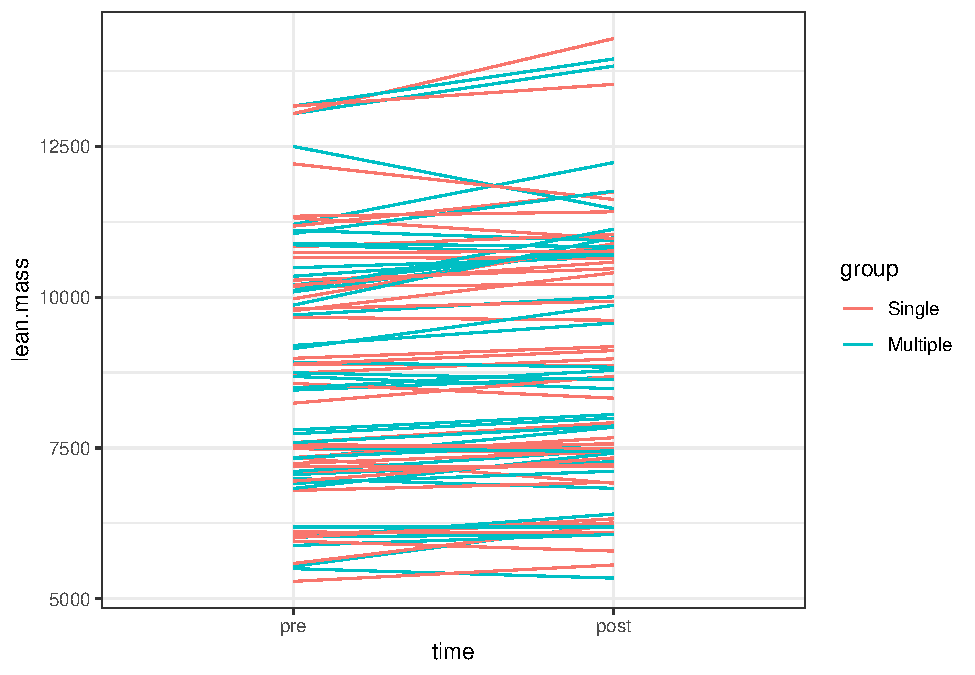
\includegraphics{_main_files/figure-latex/unnamed-chunk-5-1.pdf}
\caption{\label{fig:unnamed-chunk-5}Muskelvekst fra pretest - posttest for alle forsøkspersoner skilt ved ett- sett og tre- sett}
\end{figure}

\underline{\textbf{Muskel styrke}}
Resultatene viser at 12 ukers treningsintervensjon fører til en endring i muskelstyrke fra pre til post test på beina som gjennomførte et sett. mellom beina som gjennomførte ett sett (31,0 ± 14,2\%, p\textless0,001), og beina som gjennomførte tre sett (2,04 ± 3,71\%, p\textless{} 0,001). Endring i muskelstyrke for de ulike treningsintervensjonene ved post test er signifikant (0.029 ae, p\textless0.029).

\begin{figure}
\centering
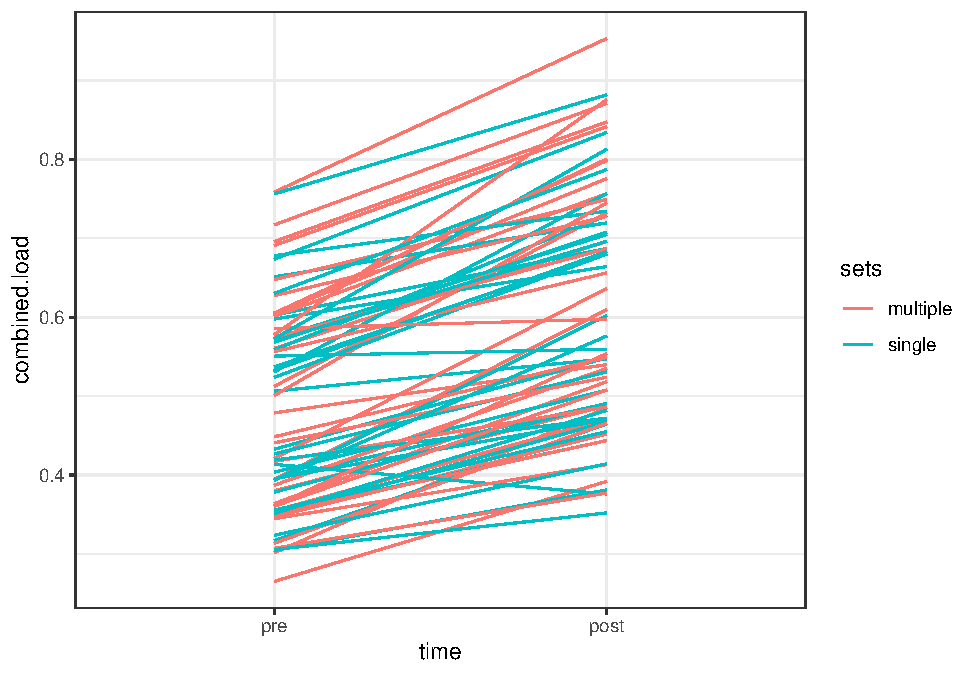
\includegraphics{_main_files/figure-latex/unnamed-chunk-7-1.pdf}
\caption{\label{fig:unnamed-chunk-7}Figur 2 viser endring i muskelstyrke for alle forsøkspersonene fra pre- post skildt ved single- sett og multiple- sett}
\end{figure}

\hypertarget{diskusjon-1}{%
\section{Diskusjon}\label{diskusjon-1}}

To til tre styrkeøkter i 12 uker øker maksimal styrke i beina, og muskel hypertrofi. Disse resultatene er gjeldende for om man gjennomfører ett eller tre sett. Resultatene presentert i denne studien viser at endringen vil være større om man gjennomfører tre sett. Dette samsvarer med det store mengder av litteraturen viser \citep{rhea2002, munn2005, fröhlich2010}. Som presentert i introduksjonen viser resultatene de presenterer at tre sett har signifikant større økning enn ett sett. Rhea med flere viser til at deltakerne som kjørte tre sett hadde dobbelt så stor utvikling som deltakerne som gjennomførte ett sett (25\%) etter tre uker (48\%). Etter 12 uker ble det større forskjell mellom gruppene hvor deltakerne som gjennomførte tre sett hadde 56\% økning, og deltakerne som gjennomførte ett sett hadde 26\% økning. Dette kan være et tegn på at skilnaden mellom gruppen kan være enda større hvis samme styrkeprogram blir gjennomført i en periode som er lengre enn 12 uker.

På den andre siden konkluderer Carpinelli \citep{carpinelli1998} som nevnt i introduksjonen at forskjellen mellom deltakerne som gjennomført ett sett og tre sett ikke var stor nok til at det var hensiktsmessig å gjennomføre tre sett. Dette understreker de med å påpeke at ved så lite forskjell vil det være lettere for folk å praktisere ett sett i sitt treningsprogram i det daglige liv. Dette er et viktig poeng å ta med seg inn i resultatene fra dette studiet da det er gjennomført på vanlige mennesker, og ikke treningsutøvere, som kan ha vanskeligheter med å få tid til å gjennomføre et styrkeprogram med tre sett på hver øvelse. Resultatene presentert over viser og at beina som gjennomførte ett sett hadde signifikant endring i lean bodymass, og i muskelstyrke.

\hypertarget{konklusjon}{%
\section{Konklusjon}\label{konklusjon}}

Etter endt studie kan man konkludere med at om man gjennomfører ett sett eller tre sett med styrketrening to til tre ganger i uken, vil man kunne se en signifikant økning i muskel styrke og hypertrofi. Ved å gjennomføre tre sett vil endringen være større enn ved ett sett. Til videre forskning kan man undersøke hvordan denne endringen vil være i en lengre periode enn 12 uker.

\hypertarget{referanser-3}{%
\section{Referanser}\label{referanser-3}}

  \bibliography{book.bib,packages.bib}

\end{document}
